%\documentclass[a4paper,landscape,twocolumn,12pt]{article}
\documentclass[a4paper,12pt]{article}

\usepackage[french]{babel}
\usepackage[utf8]{inputenc}
\usepackage[T1]{fontenc}
\usepackage{graphicx}
\usepackage{tabularx}
\usepackage{color}
\usepackage{tikz}\usetikzlibrary{shapes.geometric}
\usepackage{url}
\usepackage{import,palatino}
\usepackage{pdfpages,wrapfig,setspace}
\usepackage[margin=15mm]{geometry}

\setlength{\parskip}{\smallskipamount}
%\setlength{\parindent}{0pt}

\pagestyle{empty}
\begin{document}
\begin{center}
  {\Huge Activités sur les algorithmes}

  \bigskip
  {\Large Livret du participant}
  \vspace{-\baselineskip}
\end{center}

\large

Ce petit livre explique étape par étape comment faire son premier jeu en Snap!
Ce jeu est simple, mais quand on a compris le principe, on facilement le faire
évoluer selon ses désires. Vous trouverez d'autres activités similaire sur le
site:

\centerline{\color{blue}\url{http://www.loria.fr/~quinson/C4K}}

\bigskip\bigskip
\bigskip\bigskip

\centerline{\Large Ceci est un petit livre à construire vous-même}


Vous trouverez de ce côté les instructions de fabrication de votre
petit livre, qui se trouve de l'autre côté de la feuille. Pas besoin
de colle, uniquement de ciseaux.

\bigskip\bigskip


\noindent
\begin{minipage}[b]{.45\linewidth}

\noindent\textbf{À l'impression}, assurez-vous que le document n'est
pas remis à l'échelle. Si votre logiciel vous donne le choix, demandez
à imprimer à 100\%, sans redimensionner.

\bigskip %
\bigskip %
\noindent\textbf{Étape 1 :} Repliez en deux, puis encore en deux et
encore en deux comme sur le dessin. Les bords doivent être bien
jointifs et les plis bien marqués, dans les deux sens.


\medskip \centerline{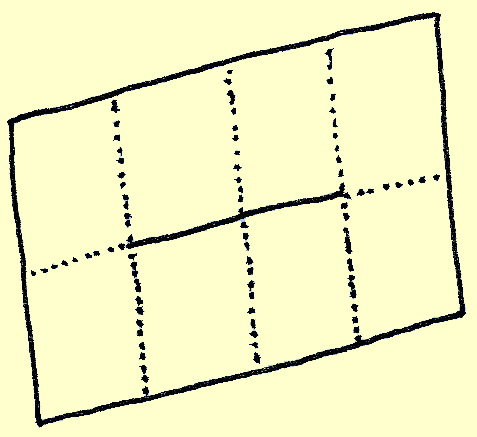
\includegraphics{img/ptitlivre-etape2.jpg}}

Si le texte est coupé par le pliage, il faut refaire l'impression sans
redimensionner le document.

\medskip

\end{minipage}\hfill\begin{minipage}[b]{.45\linewidth}
\noindent\textbf{Étape 2 :} Découpez le pli au milieu de la page.

\medskip %
\centerline{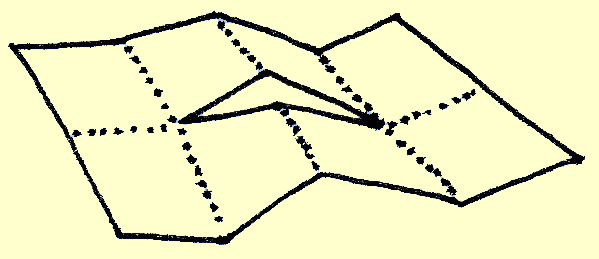
\includegraphics{img/ptitlivre-etape3.jpg}}
 
\bigskip %
\noindent\textbf{Étape 3 :} Repliez la feuille dans le sens de la longueur.\\

\centerline{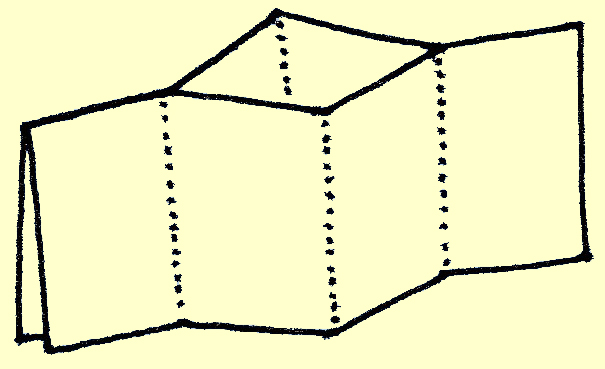
\includegraphics{img/ptitlivre-etape4.jpg}}
  
\bigskip

\noindent
\begin{minipage}{.6\linewidth}
\noindent\textbf{Étape 4 :} Repliez les deux parties centrales, repliez
le tout et c'est fini !
\end{minipage}\hfill%
\begin{minipage}{.35\linewidth}
  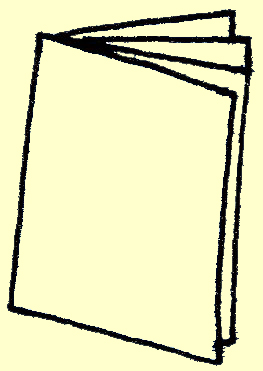
\includegraphics{img/ptitlivre-etape5.jpg}
\end{minipage}

\bigskip
\end{minipage}

\bigskip~\hfill{\small Le concept du «~petit livre~» est une idée
  originale de {\color{blue}\url{http://petitslivres.free.fr/}}}
  
\bigskip \bigskip \bigskip \normalsize %
\noindent\copyright{} 2014 Martin Quinson et Jean-Christophe Bach
(version du 18 mai 2014). \\ Libre diffusion sous licence
CC-BY-SA. Merci de nous indiquer toute amélioration possible sur:

\centerline{\color{blue}\url{https://github.com/mquinson/coding4kids}}

\end{document}
